The \texttt{component} package contains different classes that make up the user interface (UI).

Most of the classes implement the adapter pattern and wrap corresponding GWT-UI classes. 
These classes are \texttt{\lnk{Checkbox}}, \texttt{\lnk{LabeledButton}}, \texttt{\lnk{OptionBox}}, 
\texttt{\lnk{PopUpTextBox}}, \texttt{\lnk{TextField}}, \texttt{\lnk{VisualButton}} and \texttt{\lnk{WindowFocus}}.
Adapting the classes not only achieves consistent naming and functionality for the UI components
but also allows for easy mocking of the classes.

Additionally a few classes are specially designed for the Wavelength IDE. The \texttt{\lnk{Editor}} 
class is implemented by the Monaco Editor API which provides a means for advanced editor functionalities. 
\texttt{\lnk{TreeOutput}} and \texttt{\lnk{UnicodeOutput}} are both interactive visualizations of 
\texttt{\hyperref[type:edu.kit.wavelength.client.model.term.LambdaTerm]{LambdaTerm}}s. They display 
the result of a calculation to the user and also allow the user to request precises calculation steps.

By wrapping the GWT-UI classes behind an adapter, all classes in the \texttt{component} package can
be hidden behind a combination of different interfaces from the \texttt{\pkglnk{view.api}}.
%TODO was ist so toll daran, die hinter den Interfaces zu verstecken?

\begin{figure}[H]
	\centering
	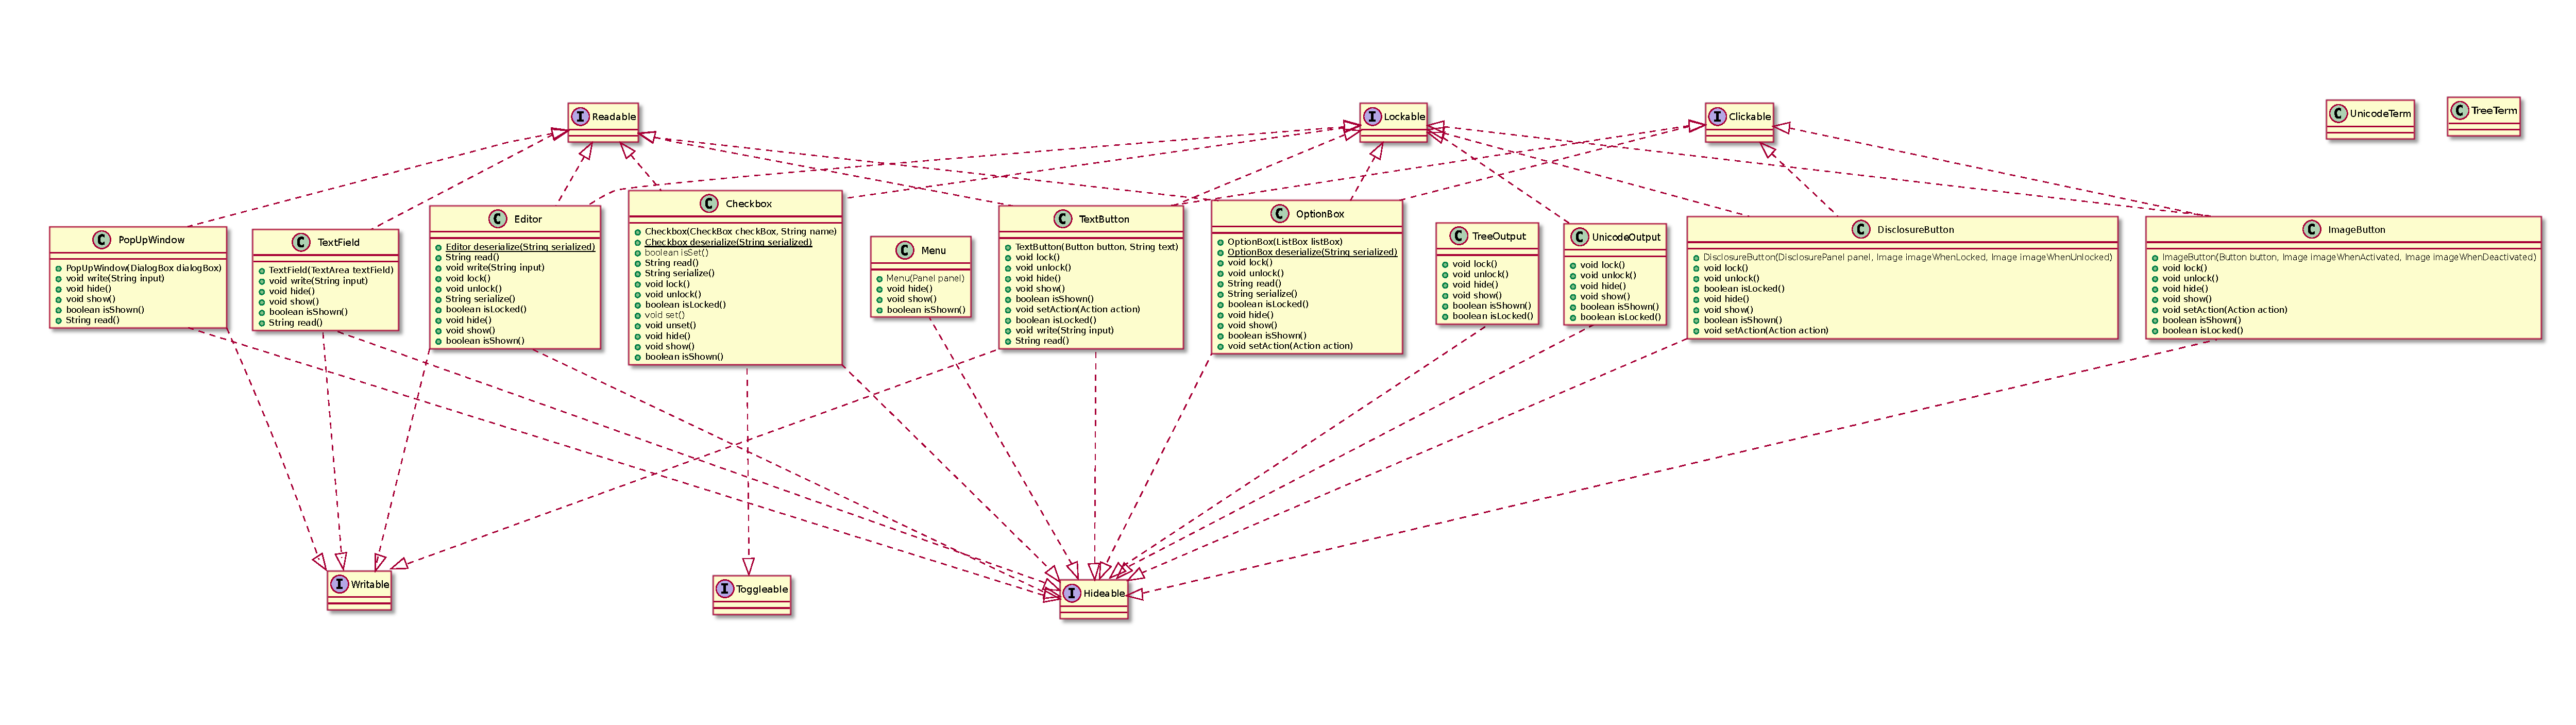
\includegraphics[width=\textwidth]{packageDiagrams/componentsPackage}
\end{figure}
